
	\emph{Dans cet exercice, chaque question est indépendante. Aucune justification n'est demandée.}
	
	\begin{enumerate}
		\item Décomposer 360 en produit de facteurs premiers.
		
		\item \begin{minipage}[t]{9 cm}
			À partir du triangle BEJ, rectangle isocèle en J, on a obtenu par pavage la figure ci-contre.
			\begin{enumerate}
				\item Quelle est l'image du triangle BEJ par la symétrie d'axe (BD) ?
				
				\item Quelle est l'image du triangle AMH par la translation qui transforme le point E en B ?
				
				\item Par quelle transformation passe-t-on du triangle AIH au triangle AMD ?
			\end{enumerate}
		\end{minipage}\hfill
		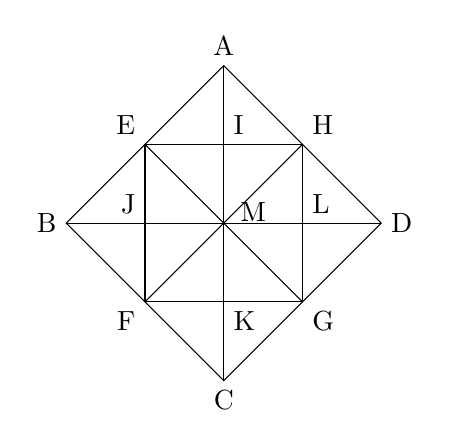
\begin{tikzpicture}[baseline={(A)}]
			\draw (0,2) node (A)[above]{A}-- (-2,0) node[left]{B} -- (0,-2) node[below] {C} -- (2,0) node[right]{D} -- cycle;
			\draw (-1,1) node[above left ]{E} -- (-1,-1) node[below left] {F} --(1,-1) node [below right] {G} -- (1,1) node [above right] {H} -- cycle;
			\draw (-2,0)--(-1,0) node[above left] {J} -- (0,0) node[shift={(20:.4)}] {M} -- (1,0) node [above right] {L}--(2,0);
			\draw (0,2)--(0,1) node[above right]{I} -- (0,-1) node[below right] {K}--(0,-2);
			\draw (-1,1)--(1,-1) (-1,-1)--(1,1);
		\end{tikzpicture}
		
		\item Calculer en détaillant les étapes : 

		$$\dfrac{7}{2} + \dfrac{15}{6} \times \dfrac{7}{25}$$
		
		On donnera le résultat sous la forme d'une fraction irréductible.
		
		\item Pour cette question, on indiquera sur la copie l'unique bonne réponse. Sachant que le diamètre de la Lune est d'environ \np[km]{3474}, la valeur qui approche le mieux son volume est :
		
		\renewcommand{\arraystretch}{1.5}
		\begin{tabularx}{\linewidth}{|*{4}{>{\centering \arraybackslash}X|}} \hline
		Réponse A     & Réponse B     &	Réponse C     &	Réponse D   \\ \hline
		$12,3 \times 10^{17}\mathrm{~km}^3$&  $\np{1456610}\mathrm{~km}^3$	&
		$1,8 \times 10^{11}\mathrm{~km}^3$ &  $2,2 \times 10^{10}\mathrm{~km}^3$ \\ \hline
		\end{tabularx}
		
		
		\item On considère un triangle RST rectangle en S. Compléter le tableau donné en ANNEXE à rendre avec la copie.
		On arrondira la valeur des angles à l'unité. 
		
	\end{enumerate}

\vspace{0,5cm}

\textbf{Annexe à rendre avec la copie - question 5 :}

\begin{tabularx}{\linewidth}{|*{4}{>{}X|}} \hline
	\textbf{Longueurs} & \textbf{Angles} & \textbf{Périmètre du triangle RST} & \textbf{Aire du triangle RST}\\ \hline
	
	\rule[-3mm]{0mm}{10mm}RS = 10 mm & $\widehat{\mathrm{RST}} = 90$° & \multirow{3}{*}{\rule{0mm}{12mm}$ \mathcal{P} = $}
	& \multirow{3}{*}{\rule{0mm}{12mm}$ \mathcal{A} = $}
	\\ \cline{1-2}
	\rule[-3mm]{0mm}{10mm}ST = 24 mm & $\widehat{\mathrm{STR}} \approx$ &&\\ \cline{1-2}
	\rule[-3mm]{0mm}{10mm}RT = 26 mm & $\widehat{\mathrm{SRT}} \approx$ &&\\ \hline
	
\end{tabularx}

